\section{Capítulo 2 Solución propuesta}

En este capítulo se presentará la solución propuesta para el desarrollo de una aplicación web destinada a la gestión de AD, abordando tanto los aspectos teóricos como técnicos involucrados en su implementación. Se comenzará detallando el modelado del negocio, incluyendo el modelo de dominio y las reglas de negocio definidas mediante patrones, seguido de un análisis de los requisitos funcionales y no funcionales. A continuación, se explicará la arquitectura del sistema, cubriendo el stack tecnológico seleccionado y los principios arquitectónicos adoptados.

Posteriormente, se procederá a describir la selección y modelado de estilos y patrones de diseño, haciendo énfasis en los principios y patrones empleados para asegurar una estructura robusta y flexible. Finalmente, se abordará la implementación de las funciones básicas, proporcionando una vista general de los componentes clave y su integración en la solución final.

\subsection{Modelado de negocio}

En este apartado se presentan tanto el modelo de dominio como las reglas del negocio organizadas por patrones. El modelo de dominio define las principales entidades y relaciones dentro del sistema, tales como usuarios, grupos, unidades organizacionales, proporcionando una representación clara del entorno de AD. Por su parte, las reglas del negocio describen los comportamientos y restricciones que deben cumplirse durante la interacción con el sistema, agrupadas según patrones que facilitan su comprensión y posterior implementación.

\subsubsection{Modelo de dominio}

El modelo de dominio representado en la \autoref{fig:domain-model} ilustra las principales entidades y relaciones involucradas en la gestión de un Directorio Activo, que es la base del sistema propuesto. Este modelo permite comprender las interacciones y dependencias entre los diferentes actores y objetos del sistema.

\begin{figure}[H]
    \centering
    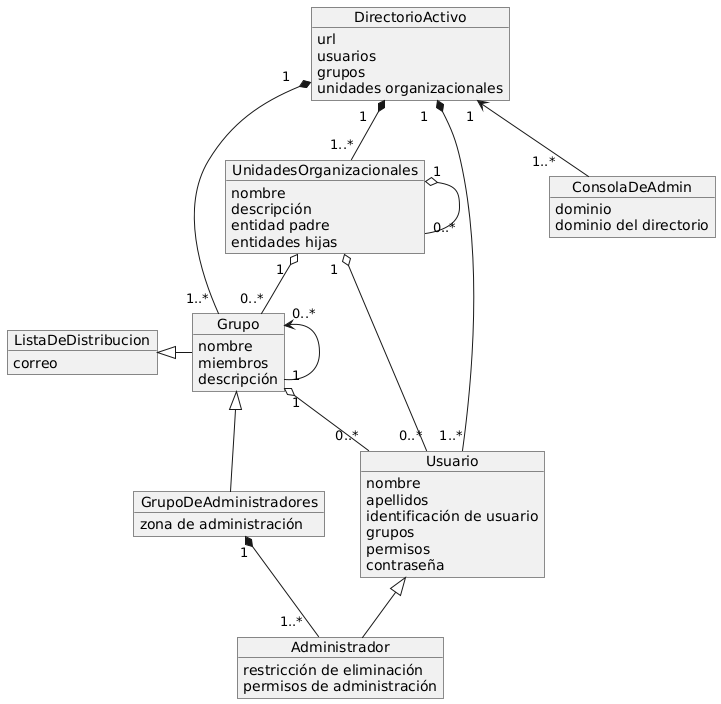
\includegraphics[width=\linewidth]{images/puml/domain-diagram/domain diagram.png}
    \caption{Modelo de dominio del sistema}
    \label{fig:domain-model}
\end{figure}
\subsubsection{Reglas del negocio por patrón}

En el desarrollo de sistemas de información, las reglas de negocio son cruciales, ya que establecen las políticas, restricciones y condiciones que guían el funcionamiento de una organización. Estas reglas resultan fundamentales para asegurar la integridad, consistencia y eficiencia de los procesos en el negocio.

La \autoref{table:bussiness-rules} muestra un resumen de las reglas de negocio identificadas hasta ahora, junto con el patrón que las representa. Esta clasificación facilita la implementación eficiente de dichas reglas en el sistema, garantizando el cumplimiento de los requisitos y expectativas del negocio.


\begin{longtable}{|p{10cm}|l|}
    \caption{Reglas del negocio}
    \label{table:bussiness-rules}                                                                                                                                                                                                                                                                                                          \\
    \hline
    \textbf{Regla}                                                                                                                                                                                                                                                                                                       & \textbf{Patrón} \\
    \hline
    \endfirsthead
    \hline
    Solo si el usuario no existe se puede crear.                                                                                                                                                                                                                                                                         & Precondición    \\ \hline
    Solo si el usuario existe se puede eliminar.                                                                                                                                                                                                                                                                         & Precondición    \\ \hline
    Solo si el usuario existe se puede editar.                                                                                                                                                                                                                                                                           & Precondición    \\ \hline
    Solo si el grupo no existe se puede crear.                                                                                                                                                                                                                                                                           & Precondición    \\ \hline
    Solo si el grupo existe se puede eliminar.                                                                                                                                                                                                                                                                           & Precondición    \\ \hline
    Solo si el grupo existe se puede editar.                                                                                                                                                                                                                                                                             & Precondición    \\ \hline
    Un grupo de tipo lista de distribución tiene: miembros, nombre, descripción y correo electrónico.                                                                                                                                                                                                                    & Estructura      \\ \hline
    Un grupo tiene: miembros, nombre, descripción.                                                                                                                                                                                                                                                                       & Estructura      \\ \hline
    Una unidad organizacional tiene: nombre y descripcion                                                                                                                                                                                                                                                                & Estructura      \\ \hline
    El administrador es responsable de la creación, edición, y eliminación de los usuarios, grupos y unidades organizacionales.                                                                                                                                                                                          & Responsablidad  \\ \hline
    El usuario debe estar autenticado para acceder a las funciones del sistema.                                                                                                                                                                                                                                          & Precondición    \\ \hline
    Solo si no se ha alcanzado el límite de usuarios, el administrador puede crear más usuarios.                                                                                                                                                                                                                         & Precondicion    \\ \hline
    Solo si no se ha alcanzado el límite de grupos, el administrador puede crear más grupos.                                                                                                                                                                                                                             & Precondición    \\ \hline
    Solo si no se ha alcanzado el límite de unidades organizacionales, el administrador puede crear más unidades organizacionales.                                                                                                                                                                                       & Precondición    \\ \hline
    Un usuario tiene nombre, apellidos, nombre de usuario, correo empresarial, correos personales, dirección, carnet de identidad, contraseña, grupos a los que pertenece, permisos, teléfono celular, telefono fijo, telefono de oficina, rol que desempeña dentro de la empresa, quién es su manager y foto de perfil. & Estructura      \\ \hline
    Si el usuario es un objeto crítico, no puede ser eliminado                                                                                                                                                                                                                                                           & Precondición    \\ \hline
    Si el grupo es un objeto crítico, no puede ser eliminado                                                                                                                                                                                                                                                             & Precondición    \\\hline
\end{longtable}



\subsection{Requisitos de la aplicación}

Este apartado describe los requisitos esenciales que deben cumplirse para el correcto funcionamiento de la aplicación web propuesta. Los requisitos funcionales especifican las principales características que permitirán la gestión de entidades en el AD, mientras que los requisitos no funcionales establecen criterios relacionados con el rendimiento, la seguridad y la usabilidad del sistema. Además, se incluye un diagrama de caso de uso para ilustrar la interacción de los usuarios con las funcionalidades clave del sistema.

\subsubsection{Casos de uso del sistema}

Los casos de uso del sistema representan las interacciones entre los actores y las funcionalidades clave de la aplicación. A través de estos, se detallan los escenarios en los que los usuarios, administradores y otros actores relevantes interactúan con el sistema para cumplir con los objetivos propuestos. A continuación en la \autoref{fig:system-use-cases-diagram}, se presenta un diagrama de caso de uso que proporciona una vista general de las acciones que los usuarios pueden realizar, contribuyendo a una mejor comprensión de los requisitos funcionales definidos.

\begin{figure}[H]
    \centering
    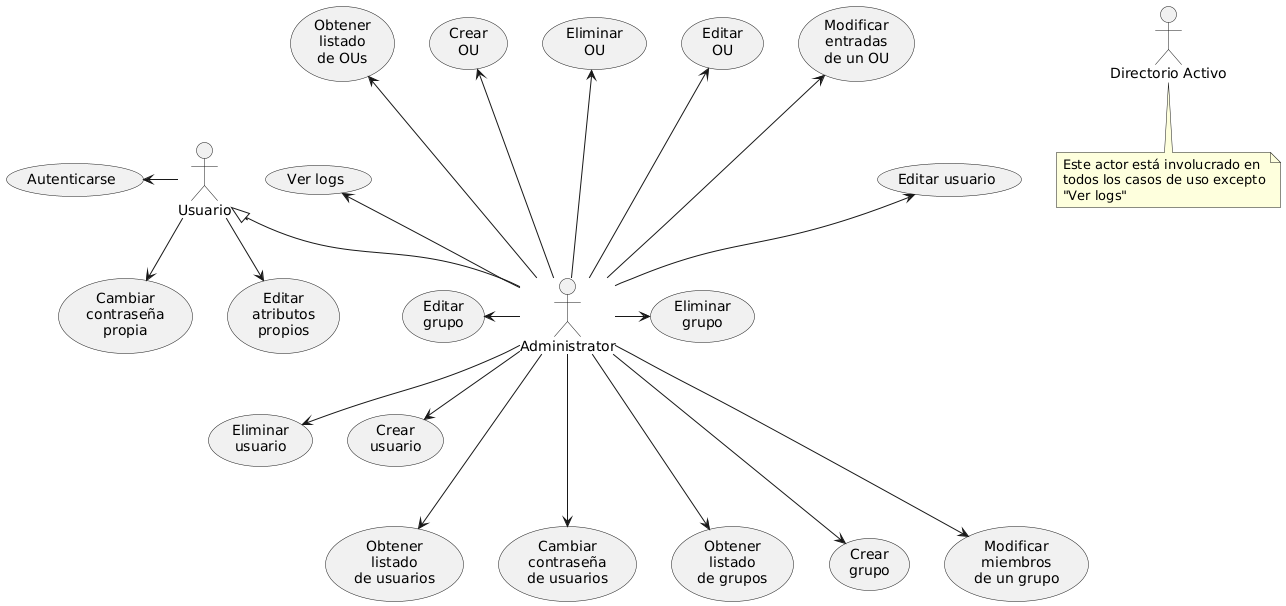
\includegraphics[width=\linewidth]{images/puml/system-diagram/system-diagram.png}
    \caption{Diagrama de casos de uso del sistema}
    \label{fig:system-use-cases-diagram}
\end{figure}
\subsubsection{Requisitos funcionales}

Los requisitos funcionales definen las funcionalidades y comportamientos que la aplicación debe ofrecer para cumplir con las necesidades del usuario y los objetivos del proyecto. En la \autoref{table:functional-requirements} a continuación se desglosan los requisitos funcionales del sistema.



\begin{longtable}{|l|p{5cm}|p{8.5cm}|}
    \caption{Requisitos funcionales del sistema}
    \label{table:functional-requirements}                                                                                                                                                                                          \\
    \hline
    \textbf{Código} & \textbf{Requisito}                                                              & \textbf{Descripción}                                                                                                       \\
    \hline
    \endfirsthead
    \textbf{RF1}   & Gestión de Usuarios: Creación de usuarios                                       & La aplicación debe permitir la creación de nuevas cuentas de usuario en el AD.                                             \\ \hline
    \textbf{RF2}   & Gestión de Usuarios: Modificación de usuarios                                   & Los administradores deben poder actualizar la información de los usuarios, como nombres, correos electrónicos, roles, etc. \\ \hline
    \textbf{RF3}   & Gestión de Usuarios: Eliminación de usuarios                                    & La aplicación debe permitir la eliminación segura de cuentas de usuario.                                                   \\ \hline
    \textbf{RF4}   & Gestión de Usuarios: Asignación de roles y permisos                             & Debe ser posible asignar y modificar roles y permisos a los usuarios para definir su nivel de acceso a los recursos.       \\ \hline
    \textbf{RF5}   & Gestión de Grupos: Creación de grupos                                           & Permitir la creación de nuevos grupos en el AD.                                                                            \\ \hline
    \textbf{RF6}   & Gestión de Grupos: Modificación de grupos                                       & Posibilidad de añadir o remover usuarios de grupos existentes.                                                             \\ \hline
    \textbf{RF7}   & Gestión de Grupos: Eliminación de grupos                                        & Permitir la eliminación de grupos.                                                                                         \\ \hline
    \textbf{RF8}   & Gestión de Unidades Organizacionales (OU): Creación de OU                       & La aplicación debe permitir la creación de nuevas Unidades Organizacionales dentro del AD.                                 \\ \hline
    \textbf{RF9}   & Gestión de Unidades Organizacionales (OU): Modificación de OU                   & Los administradores deben poder renombrar y mover OUs dentro de la jerarquía del directorio.                               \\ \hline
    \textbf{RF10}  & Gestión de Unidades Organizacionales (OU): Eliminación de OU                    & Debe ser posible eliminar OUse.                                                                                            \\ \hline
    \textbf{RF11}  & Gestión de Unidades Organizacionales (OU): Asignación de usuarios y grupos a OU & La aplicación debe facilitar la asignación de usuarios y grupos a las OUs para una mejor organización dentro del AD.       \\ \hline
    \textbf{RF12}  & Autenticación y Autorización: Integración con LDAP                              & La aplicación debe autenticarse a través de LDAP con el AD para validar usuarios y permisos.                               \\ \hline
    \textbf{RF13}  & Autenticación y Autorización: Gestión de sesiones                               & Manejo de sesiones de usuario con opciones de inicio y cierre de sesión seguro.                                            \\ \hline
    \textbf{RF14}  & Auditoría y Registro de Actividades: Registro de eventos                        & La aplicación debe registrar todas las operaciones realizadas sobre los usuarios, grupos y OUs, incluyendo quién y cuándo. \\ \hline
    \textbf{RF15}  & Interfaz de Usuario (UI): Consola de administración                             & Proveer una interfaz amigable y accesible para la gestión de usuarios, grupos, OUs y revisión del registro de eventos.     \\ \hline
    \textbf{RF16}  & Interfaz de Usuario (UI): Notificaciones                                        & Mostrar notificaciones en la UI para confirmar la ejecución exitosa de acciones o para advertir sobre errores.             \\ \hline
    \textbf{RF17}  & Configuración de la Aplicación: Facilidad de configuración                      & La aplicación debe ser fácilmente configurable a través de archivos .json o .yaml, validados mediante JSON Schema.         \\ \hline
\end{longtable}

\subsubsection{Requisitos no funcionales}

Los requisitos no funcionales describen las cualidades que debe tener la aplicación para garantizar un desempeño óptimo y satisfacer las expectativas de los usuarios. En la \autoref{table:non-functional-requirements} se enumeran los requisitos funcionales que debe presentar el sistema.


\begin{longtable}{|l|l|p{12cm}|}
    \caption{Requisitos no funcionales del sistema}
    \label{table:non-functional-requirements}                                                                                                                                                 \\
    \hline
    \textbf{Código} & \textbf{Requisito} & \textbf{Descripción}                                                                                                                               \\
    \hline
    \endfirsthead
    \textbf{RNF1}   & Calidad            & La aplicación debe ser capaz de manejar un creciente número de usuarios y grupos sin degradación significativa en el rendimiento.                  \\ \hline
    \textbf{RNF2}   & Restricción        & La aplicación debe implementar mecanismos de seguridad como cifrado de datos, autenticación segura, y control de acceso basado en roles (RBAC).    \\ \hline
    \textbf{RNF3}   & Calidad            & Las operaciones críticas como la autenticación y la gestión de usuarios deben completarse en menos de 2 segundos en condiciones normales de carga. \\ \hline
    \textbf{RNF4}   & Calidad            & La interfaz debe ser intuitiva y fácil de usar, con una curva de aprendizaje mínima para administradores y usuarios avanzados.                     \\ \hline
    \textbf{RNF5}   & Restricción        & La aplicación debe ser compatible con múltiples navegadores web modernos y adaptarse a diferentes tamaños de pantalla (responsive design).         \\ \hline
    \textbf{RNF6}   & Calidad            & El código debe ser modular y bien documentado, facilitando futuras actualizaciones y correcciones de errores.                                      \\ \hline
    \textbf{RNF7}   & Calidad            & La configuración de la aplicación debe estar documentada de manera clara y accesible, disponible en línea en el sitio web del proyecto.            \\ \hline
    \textbf{RNF8}   & Restricción        & La aplicación debe ser web                                                                                                                         \\ \hline
    \textbf{RNF9}   & Restricción        & La aplicacion debe ser de código abierto                                                                                                           \\ \hline
\end{longtable}


\subsection{Arquitectura de la aplicación web}

En esta sección se aborda la arquitectura de la aplicación web propuesta, describiendo su estructura general, los patrones arquitectónicos adoptados y el stack tecnológico utilizado. La arquitectura de la aplicación se diseña con el objetivo de proporcionar una solución escalable, mantenible y eficiente para la gestión de AD. Se detalla la elección de tecnologías así como los problemas frecuentes y su solución.

\subsubsection{Stack tecnológico}

El stack tecnológico elegido para el desarrollo de la aplicación fue fundamental para garantizar tanto el rendimiento como la mantenibilidad del sistema. A continuación, se describen los componentes principales del stack:


\textbf{Framework de desarrollo: SvelteKit}

SvelteKit se ha seleccionado como el framework principal debido a su capacidad para crear aplicaciones rápidas con una experiencia de desarrollo eficiente. SvelteKit ofrece ventajas como el renderizado en el lado del servidor (SSR), la generación de sitios estáticos (SSG), y una integración sencilla con herramientas modernas como Vite. Además, su enfoque en la eliminación del tiempo de ejecución permite que las aplicaciones sean ligeras y rápidas, lo cual es esencial para la experiencia del usuario.

\textbf{Cliente LDAP: ldapts}

Para la comunicación con el servidor LDAP, se ha optado por ldapts, un cliente LDAP para Node.js que ofrece una API asincrónica basada en promesas y con soporte para typescript. Esta herramienta es ideal para interactuar con AD, permitiendo operaciones como búsqueda, adición, modificación y eliminación de entradas en el directorio. Su uso simplifica la integración de LDAP en la aplicación, garantizando la seguridad y eficiencia necesarias para la gestión de usuarios.

\subsubsection{Problemas frecuentes y soluciones en la arquitectura de la aplicación}

Este epígrafe aborda los problemas comunes que pueden surgir en el desarrollo de aplicaciones web y presenta soluciones basadas en la arquitectura adoptada. Se exploran aspectos clave como la seguridad, el rendimiento, la escalabilidad y la integración de servicios externos, destacando cómo la elección adecuada de tecnologías puede ayudar a mitigar estos desafíos.

\textbf{Integración de APIs y servicios externos}: las aplicaciones web a menudo requieren la integración con servicios externos. En este caso, la única integración externa es con AD, que se realiza a través del cliente LDAP proporcionado por la librería ldapts. Esta librería permite una conexión eficiente con el directorio, aprovechando su naturaleza asíncrona para mejorar el rendimiento y los tiempos de carga.

\textbf{Rendimiento y tiempos de carga}: problemas de rendimiento y tiempos de carga pueden afectar la experiencia del usuario. SvelteKit, con su enfoque de generación de sitios estáticos y pre-renderización, ayuda a mejorar la velocidad de carga. La integración con ldapts, una librería asíncrona para la comunicación con AD, mejora el rendimiento al manejar operaciones de directorio de manera eficiente sin bloquear el hilo principal. Esto asegura que las consultas LDAP no impacten negativamente en el rendimiento global de la aplicación.

\textbf{Escalabilidad y mantenibilidad}: con el crecimiento de la aplicación, la escalabilidad y mantenibilidad son esenciales. La arquitectura en capas implementada con SvelteKit facilita una separación clara de responsabilidades, mejorando la organización y la evolución del código. La capa de presentación, la capa de negocio y la capa de datos están claramente definidas, permitiendo un desarrollo modular y la fácil adaptación a nuevas funcionalidades. Esta estructura en capas asegura que la aplicación pueda escalar de manera efectiva y mantenerse fácilmente a medida que se amplían los requisitos.

\textbf{Seguridad de la información y acceso}: La gestión de identidades y el control de acceso son esenciales para asegurar la aplicación web. La integración con AD a través del cliente LDAP de ldapts permite una autenticación centralizada y segura para los usuarios. Para reforzar la seguridad, se utiliza LDAPS (LDAP sobre SSL/TLS), que cifra la comunicación entre la aplicación y el servidor LDAP, protegiendo los datos de autenticación y los permisos de acceso contra interceptaciones y ataques. Este enfoque garantiza un manejo riguroso de credenciales y permisos, manteniendo la integridad y confidencialidad de la información.
\subsection{Selección y modelado de estilos y patrones}

Los estilos arquitectónicos guían la composición y relación de los componentes en un sistema de software. A continuación, se presentan brevemente los estilos seleccionados para la implementación de la solución.

\textbf{Estilo Llamada-Retorno}

El sistema sigue un enfoque de "Llamada-Retorno", donde las capas del sistema se comunican a través de llamadas y retornos de resultados. Esto se aplica a la interacción entre la capa de presentación, la capa de lógica de negocio y la capa de acceso a datos (\autoref{fig:call-return-style}), asegurando una separación clara de responsabilidades y facilitando la escalabilidad y mantenibilidad del software.

En la \autoref{fig:call-return-style-example} se muestra un ejemplo de puesta en práctica de este estilo en el sistema, donde la capa de lógica de negocio \underline{llama} a la función \textbf{getDirectChildren} de de la capa de acceso a datos, la cual \underline{retorna} los hijos directos de una entrada  del directorio.

\begin{figure}[th]
    \centering
    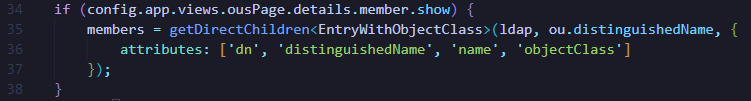
\includegraphics[width=\linewidth]{images/code/getDirectChildren-call.png}
    \caption{Ejemplo del estilo Llamada-Retorno en el sistema}
    \label{fig:call-return-style-example}
\end{figure}

\textbf{Patrón Cliente-Servidor}

El sistema implementa el patrón Cliente-Servidor, donde el cliente (la interfaz de usuario) se comunica con el servidor para solicitar servicios o datos. Este patrón facilita la separación de responsabilidades y la escalabilidad del sistema. Esta comunicación se realiza en su mayoría mediante el envío de formularios.

\textbf{Patrón de Acceso a Datos}

Para la gestión de los datos en el sistema, se implementa el Patrón de Acceso a Datos como un intermediario entre los servicios de la aplicación y el AD. Específicamente, este patrón facilita las siguientes operaciones:
\begin{itemize}
    \item \textbf{Abstracción del AD}: Se usa la librería ldapts, que abstrae las interacciones con el AD, simplificando el código y reduciendo errores.
    \item \textbf{Centralización de acceso}: Todas las solicitudes de datos pasan por esta capa, asegurando un flujo controlado y consistente.
    \item \textbf{Seguridad centralizada}: La capa implementa políticas de seguridad uniformes para todas las operaciones en el AD.
\end{itemize}

En la \autoref{fig:using-ldap-client-to-search-in-directory} muestra la declaración de la función \textbf{getDirectChildren} mencionada anteriormente, donde se utiliza el cliente ldap (de la librería ldapts) para realizar una búsqueda en el directorio. El uso del cliente ldap abstrae la interacción con el directorio además de centralizar el acceso.

\begin{figure}[H]
    \centering
    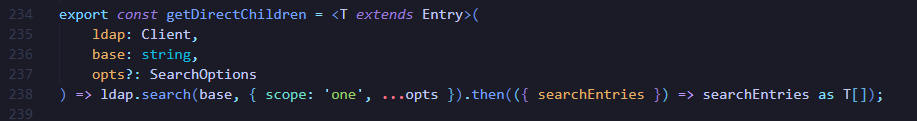
\includegraphics[width=\linewidth]{images/code/getDirectChildren.png}
    \caption{Uso del cliente ldap para realizar una búsqueda en el directorio}
    \label{fig:using-ldap-client-to-search-in-directory}
\end{figure}

\textbf{Patrón n-capas}
La arquitectura del sistema está organizada en un patrón de n-capas (\autoref{fig:n-layer-system-structure}), con una capa de presentación que interactúa con la capa de lógica de negocio, la cual a su vez se comunica con la capa de acceso a datos. Este enfoque modulariza las responsabilidades y mejora la escalabilidad y mantenibilidad del sistema.

\begin{figure}[H]
    \centering
    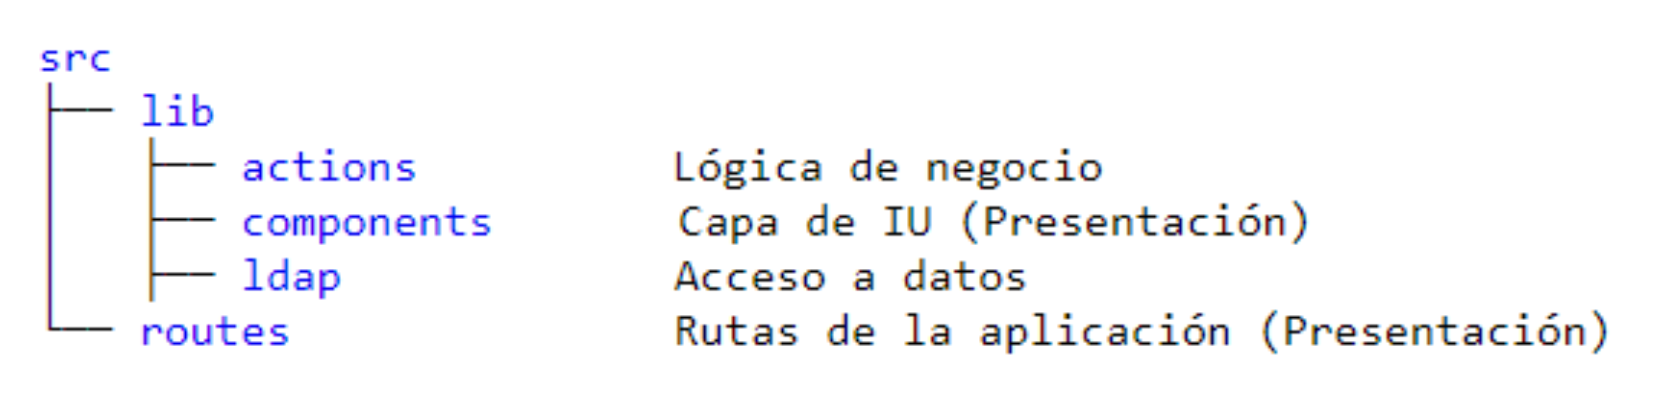
\includegraphics[width=\linewidth]{images/app-folder-structure.png}
    \caption{Estructura simplificada del sistema mostrando n-capas}
    \label{fig:n-layer-system-structure}
\end{figure}
\subsection{Principios de diseño}

\textbf{Principio de responsabilidad única}

El Principio de Responsabilidad Única (SRP, por sus siglas en inglés) es uno de los principios SOLID de diseño de software. Según SRP, una clase o módulo debería tener una única razón para cambiar, es decir, debería tener una única responsabilidad o propósito.

En el sistema se tienen varios módulos que funcionan de manera independiente y tienen un único propósito, en la \autoref{fig:bussiness-logic-modules} se muestran algunos de estos módulos cuyas responsabilidades son la autenticación, la gestión de grupos, la gestion de unidades organizacionales, el manejo de las operaciones directas sobre el árbol del directorio, y la gestión de usuarios respectivamente (\autoref{fig:collapsed-view-of-user-module}).

\begin{figure}[H]
    \centering
    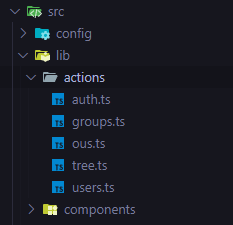
\includegraphics{images/code/bussiness-logic-modules.png}
    \caption{Módulos de la capa de logica de negocio}
    \label{fig:bussiness-logic-modules}
\end{figure}

\textbf{Principio Hollywood (Principio de Inversión de Control)}

Los módulos de alto nivel no deben depender de módulos de bajo nivel. Los módulos de bajo nivel deben depender de módulos de alto nivel. Los módulos de bajo nivel deben ser "llamados" por módulos de alto nivel y no al revés.

El diagrama de secuencia en la \autoref{fig:general-form-submission-diagram} ilustra cómo se lleva a cabo el procesamiento de una solicitud de envío de formulario en la arquitectura de n-capas del sistema, destacando la implementación del Principio de Inversión de Control (IoC).

La lógica de negocio delega la interacción con el AD al servicio de acceso a datos, siguiendo el Principio de Inversión de Control. Esto asegura que los módulos de alto nivel no dependan directamente de los módulos de bajo nivel, mejorando la flexibilidad y mantenibilidad del sistema.

\textbf{Principio Abierto-Cerrado}

El Principio Abierto-Cerrado establece que un módulo debe estar abierto para su extensión pero cerrado para su modificación. Este principio, aunque tradicionalmente asociado a la programación orientada a objetos, también es aplicable en la arquitectura de componentes en Svelte.

En lugar de modificar directamente el comportamiento de un componente, se sugiere su extensión mediante la creación de nuevos componentes o la utilización de la composición. Esto permite la introducción de nuevas funcionalidades sin alterar el código fuente original, preservando la estabilidad y confiabilidad del sistema.

Este principio se aplica en la manera en que los componentes de Svelte están diseñados para ser reutilizables y componibles. Un ejemplo claro se presenta en la \autoref{fig:open-closed-slots}, muestra cómo un mismo componente Input en Svelte puede adaptarse a través del uso de diferentes propiedades (props) y ranuras (slots), permitiendo su reutilización en distintos contextos sin necesidad de modificar su implementación base.

\begin{figure}[H]
    \centering
    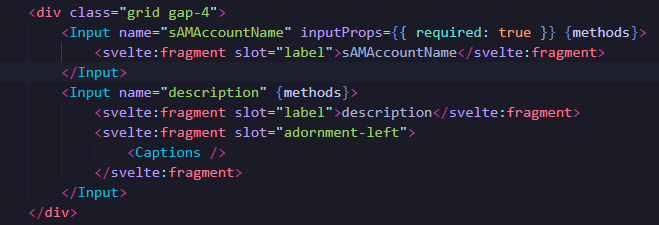
\includegraphics[width=\linewidth]{images/code/open-closed-slots.png}
    \caption{Instancias del componente Input ilustrando el pincipio Abierto-Cerrado mediante la composición de componentes}
    \label{fig:open-closed-slots}
\end{figure}
\subsection{Patrones de diseño}

En el desarrollo de software, los patrones de diseño son soluciones probadas y reutilizables para problemas comunes que los desarrolladores enfrentan al diseñar aplicaciones.

\textbf{Patrón de Convención sobre Configuración (CoC)}

El sistema adopta el Patrón CoC, que permite gestionar configuraciones a través de archivos externos. Esta práctica facilita la personalización y la flexibilidad, permitiendo ajustes sin necesidad de modificar el código fuente. Esto es crucial para adaptar la aplicación a diferentes entornos y necesidades organizacionales, mejorando la mantenibilidad y escalabilidad del sistema.

En la implementación del Patrón de CoC, se establecieron valores predeterminados para la configuración LDAP y otros aspectos. Se implementó soporte para archivos de configuración en formato JSON y YAML, validados mediante JSON Schema, para permitir ajustes específicos. Esta aproximación no solo facilita la configuración inicial de la aplicación, sino que también ofrece flexibilidad para personalizar la configuración según los requisitos del usuario final.

\textbf{Patrón de Observador}
El Patrón Observador es una técnica de diseño fundamental en el desarrollo de software para establecer relaciones de dependencia. En este patrón, cuando un objeto cambia su estado, todos los objetos dependientes son notificados y actualizados automáticamente.

En el contexto de SvelteKit, el patrón Observador es crucial para la gestión de la reactividad a través de los stores. En la \autoref{fig:loader-store-reaction} se muestra un componente que solo es visible si el valor de la store \textbf{loading} de la \autoref{fig:loader-store-declaration} tiene valor \textbf{true}. Por lo tanto cualquier componente que se modifique el valor de esta store provoca una mutación en el estado del componente de la \autoref{fig:loader-store-reaction}.

\begin{figure}[H]
    \centering
    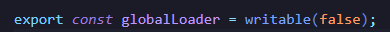
\includegraphics[width=\linewidth]{images/code/loader-store-declaration.png}
    \caption{Declaracion de un store en Sveltekit}
    \label{fig:loader-store-declaration}
\end{figure}

\begin{figure}[H]
    \centering
    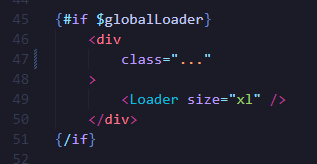
\includegraphics{images/code/loader-store-reaction.png}
    \caption{Reacción al cambio en la store}
    \label{fig:loader-store-reaction}
\end{figure}

\textbf{Patrón inyeccion de dependencias}

El patrón de Inyección de Dependencias es un patrón de diseño que busca mejorar la modularidad y la reutilización del código al desacoplar la creación de objetos de su uso. En lugar de que una clase o módulo cree directamente sus dependencias, estas son proporcionadas desde el exterior.

La \textit{Context API}(API de contexto) de Svelte es una herramienta que facilita la comunicación entre componentes sin necesidad de pasar propiedades a través de cada nivel del árbol de componentes. Este mecanismo se utiliza para compartir datos y servicios globales dentro de una aplicación, lo que permite una gestión más eficiente de las dependencias y contribuye a un diseño más limpio y modular.

En el contexto del sistema, la API de contexto se utiliza para inyectar la configuración de la aplicación relacionada con la página actual (\autoref{fig:context-api-dep-injection}). Esto permite que los componentes accedan a la configuración específica de la página sin necesidad de recibirla a través de props (\autoref{fig:context-api-usage}).

\begin{figure}[H]
    \centering
    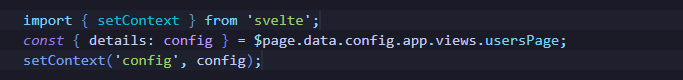
\includegraphics[width=\linewidth]{images/code/context-api-dep-injection.png}
    \caption{Uso de la API de Contexto de Sveltekit para inyectar la configuración de la página}
    \label{fig:context-api-dep-injection}
\end{figure}

\begin{figure}[H]
    \centering
    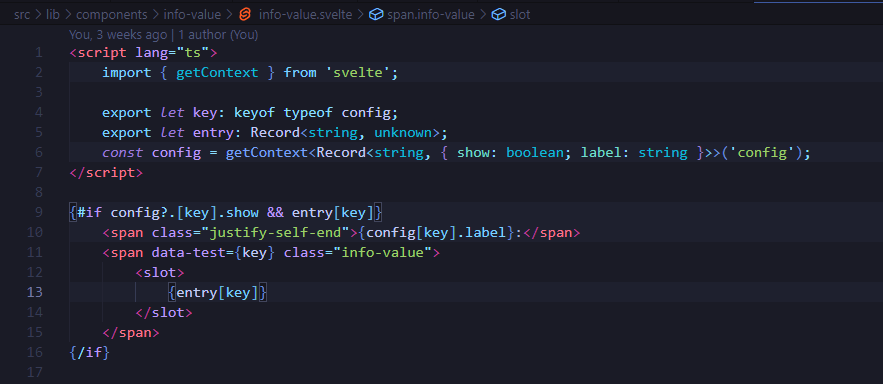
\includegraphics[width=\linewidth]{images/code/context-api-usage.png}
    \caption{Uso de la API de Contexto de Sveltekit para leer la configuracion de la página}
    \label{fig:context-api-usage}
\end{figure}
\subsection{Implementación}

En esta sección se abordarán las funciones fundamentales implementadas en la aplicación web para la gestión y autenticación de usuarios basada en AD. Estas funciones son esenciales para garantizar una operación eficiente y segura del sistema.

\subsubsection{Configuración del cliente LDAP seleccionado}

La configuración del cliente LDAP es crucial para la comunicación efectiva entre la aplicación web y el AD. En esta sección, se detallará el proceso de configuración del cliente LDAP seleccionado, ldapts.

\textbf{Creación de la instancia del cliente}

La creación de la instancia del cliente LDAP (\autoref{fig:ldap-client-initialization}) es un proceso modular que permite incorporar opciones de configuración personalizadas. La función \textbf{getLDAPClient} , la toma las opciones por defecto de la configuración del sistema, definida en el objeto \textbf{config}, y permite la sobrescritura de parámetros mediante el uso de la función \textbf{deepmerge}. De este modo, se asegura flexibilidad en la configuración sin comprometer las configuraciones base.

\begin{figure}[h]
    \centering
    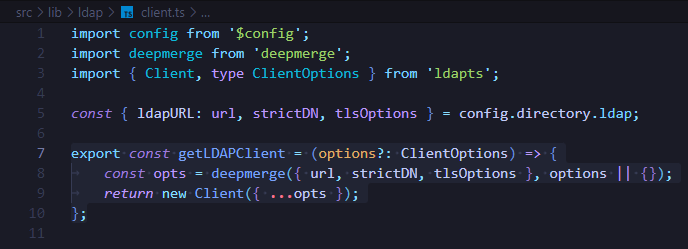
\includegraphics[width=\linewidth]{images/code/ldap-client-initialization.png}
    \caption{Creación del cliente LDAP con ldapts}
    \label{fig:ldap-client-initialization}
\end{figure}

En el fragmento de código de la \autoref{fig:ldap-client-initialization}, se extraen las configuraciones necesarias para la conexión con el AD (como url, strictDN y tlsOptions) y se combinan con las opciones adicionales que se pueden pasar al crear la instancia del cliente LDAP.

\textbf{Manejadores de autenticación}

Para asegurar una operación segura y eficiente del cliente LDAP durante el ciclo de vida de las solicitudes HTTP en la aplicación, se implementaron dos manejadores (handlers) clave en el archivo \textit{src/hooks.server.ts}:
\begin{itemize}
    \item \textbf{authenticationSetHandler}: Este manejador se encarga de inyectar una función de autenticación en las variables locales del evento. Esta función, llamada auth, valida la presencia de un token de acceso y un token de sesión, y si ambos son válidos, realiza la operación bind con el cliente LDAP, utilizando las credenciales del usuario autenticado (\autoref{fig:authentication-set-handler}).
    \item \textbf{ldapUnbindHandler}: Este manejador asegura que el cliente LDAP cierre correctamente la conexión después de procesar cada solicitud, mediante la operación unbind, liberando así los recursos de forma segura y evitando conexiones abiertas innecesarias (\autoref{fig:ldap-unbind-handler}).
\end{itemize}

Este enfoque garantiza que el cliente LDAP esté disponible solo cuando se necesita y que se libere de manera adecuada al final de cada solicitud, lo que mejora tanto la seguridad como el rendimiento general del sistema. Al centralizar la desconexión en un solo lugar, se garantiza que el cliente siempre se cierre adecuadamente después de cada solicitud, evitando conexiones abiertas que podrían saturar el sistema o generar problemas de seguridad. Esta práctica contribuye a una gestión más eficiente y segura del ciclo de vida del cliente LDAP.

\subsubsection{Desarrollo de mecanismos de autenticación}

La autenticación es una de las funciones más críticas en el sistema, ya que asegura que los usuarios solo puedan acceder a la aplicación con credenciales válidas en el AD. A continuación, se describen los mecanismos de autenticación desarrollados, destacando las interacciones con el AD y el uso de tokens para la gestión de sesiones.

\textbf{Manejadores de autenticación}

Como se explicó en secciones anteriores, los manejadores (handlers) authenticationSetHandler (\autoref{fig:authentication-set-handler})  y ldapUnbindHandler (\autoref{fig:ldap-unbind-handler}) juegan un papel crucial en la gestión de la autenticación. Estos aseguran que las conexiones al AD se establezcan y se liberen correctamente tras cada solicitud, manteniendo el sistema seguro y eficiente.

\textbf{Proceso de inicio de sesión}

El proceso de autenticación se basa en la operación \textbf{bind} proporcionada por el cliente LDAP. Este proceso se gestiona en el módulo de autenticación, método \textbf{signIn}, encargado de validar las credenciales del usuario y establecer las cookies de sesión. En la \autoref{fig:flow-diagram-auth-method} se muestra el diagrama de flujo detallando los pasos seguidos por el método:
\begin{enumerate}
    \item \textbf{Validación del formulario y captcha}: El sistema recibe los datos del formulario de inicio de sesión y valida tanto las credenciales del usuario como el token de captcha para prevenir intentos de acceso automatizados y ataques de fuerza bruta.
    \item \textbf{Autenticación en el AD}: Una vez que el captcha y las credenciales del usuario se validan correctamente, el sistema intenta autenticar al usuario en el AD a través del cliente LDAP. Si la autenticación falla, se maneja de acuerdo con los diferentes códigos de error que proporciona el AD, permitiendo mensajes de error detallados como "Credenciales inválidas", "Cuenta deshabilitada", o "Contraseña expirada".
    \item \textbf{Generación de tokens y cookies}: Si la autenticación es exitosa, el sistema recupera la entrada del usuario en el AD y genera los tokens de sesión y acceso. Estos tokens se almacenan en cookies para futuras solicitudes.
    \item \textbf{Redirección del usuario}: Una vez completado el proceso de inicio de sesión, el sistema redirige al usuario a su página de perfil.
\end{enumerate}

\begin{figure}[H]
    \centering
    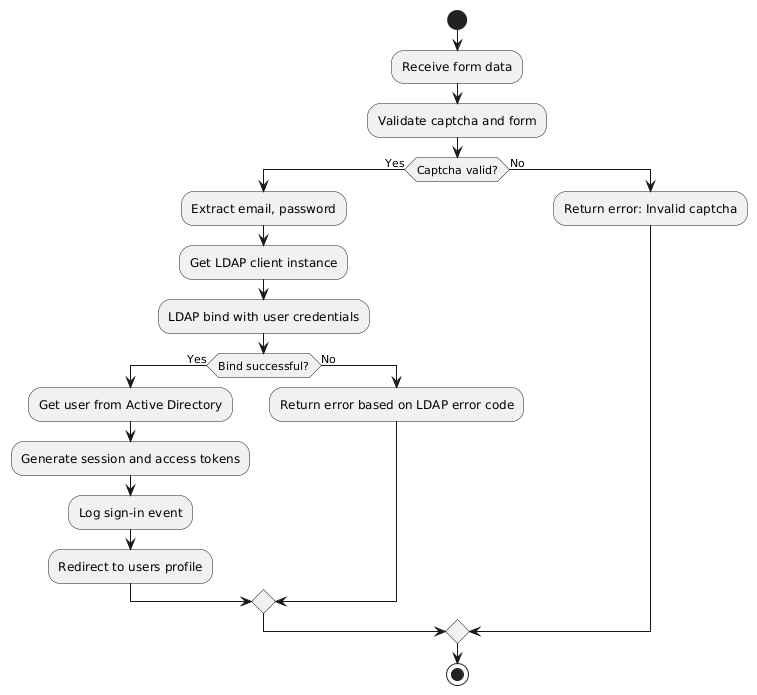
\includegraphics[scale=0.5]{images/puml/flow-diagram-signin/flow-diagram signin.png}
    \caption{Diagrama de flujo: Función de autenticación}
    \label{fig:flow-diagram-auth-method}
\end{figure}

\textbf{Proceso de cierre de sesión}

Este proceso se gestiona en el módulo de autenticación, método signOut, que elimina las cookies de sesión y acceso, invalidando así la sesión del usuario. Este mecanismo asegura que, tras cerrar la sesión, el usuario ya no podrá acceder a la aplicación hasta que vuelva a autenticarse correctamente (\autoref{fig:flow-diagram-signout-method}).

\begin{figure}[H]
    \centering
    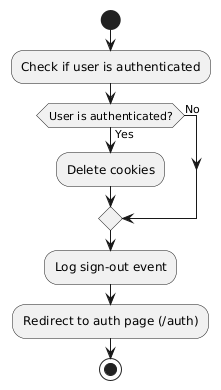
\includegraphics[scale=0.6]{images/puml/flow-diagram-signout/flow-diagram signout.png}
    \caption{Diagrama de flujo: Función cerrar sesión}
    \label{fig:flow-diagram-signout-method}
\end{figure}

\subsubsection{Flujos de gestión}

Los flujos de gestión definen el ciclo de vida de los objetos del Directorio en la aplicación, asegurando que las operaciones realizadas por los administradores se sincronicen correctamente con el AD. Estas operaciones incluyen la creación, lectura, actualización y eliminación de objetos.

\textbf{Creación de objetos}

Cuando un nuevo objeto, como un usuario o grupo, es creado desde la aplicación, este es registrado en el AD mediante una operación add (\autoref{fig:ldap-add-operation}). El cliente LDAP, ldapts, se utiliza para establecer una conexión segura y confiable con el servidor del AD, donde se envían los atributos requeridos para el nuevo objeto. A lo largo del proceso, se validan los datos, y cualquier error encontrado es notificado al usuario tal y como se muestra en la \autoref{fig:activity-diagram-create-user}.

\begin{figure}[H]
    \centering
    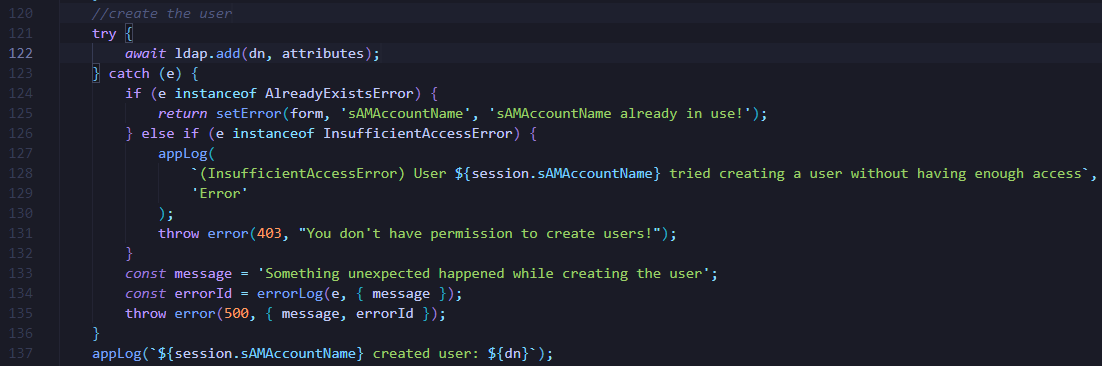
\includegraphics[width=\linewidth]{images/code/ldap-add-operation.png}
    \caption{Uso de la operacion \textit{add} con el cliente LDAP}
    \label{fig:ldap-add-operation}
\end{figure}

\textbf{Lectura de objetos}

La lectura de objetos permite a los administradores consultar los detalles de los usuarios, grupos y otros elementos en el AD. Esta operación se realiza mediante el cliente LDAP utilizando la función de búsqueda, filtrando los resultados con base en los parámetros establecidos. Los administradores pueden visualizar los detalles de los objetos, incluidas sus propiedades y relaciones con otros objetos. En la \autoref{fig:get-all-users} se muestra la función getAllUsers donde se utiliza la operación search aplicando determinados filtros para obtener las entradas del directorio que sean del esquema usuario.

\begin{figure}[H]
    \centering
    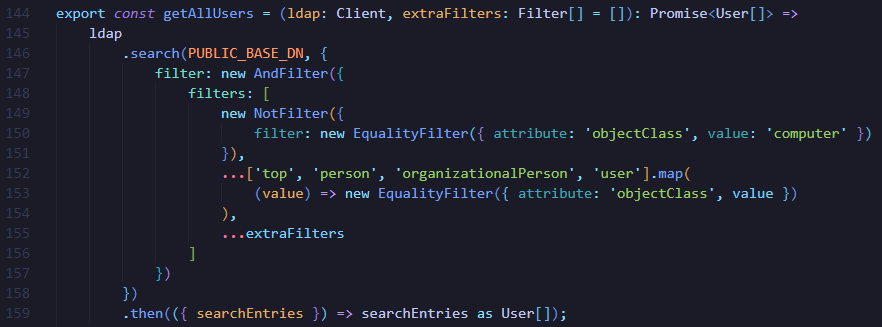
\includegraphics[width=\linewidth]{images/code/getAllUsers.png}
    \caption{Uso de la operación \textit{search} del cliente LDAP para listar usuarios}
    \label{fig:get-all-users}
\end{figure}

\textbf{Actualización de objetos}

La actualización de objetos en el AD se gestiona a través de operaciones \textbf{modify} o \textbf{replace}. La aplicación permite a los administradores modificar los atributos de los objetos, como los datos personales de un usuario o la membresía de un grupo. Una vez validados los cambios, estos se aplican directamente al AD, asegurando que la información sea precisa y esté actualizada. En la \autoref{fig:flow-diagram-update-group} se detalla el flujo de actualización de un grupo.

\textbf{Eliminación de objetos}

Finalmente, la eliminación de objetos se maneja mediante una operación delete. Los administradores pueden eliminar usuarios, grupos o unidades organizativas, y el cambio se refleja de inmediato en el AD. Antes de la eliminación, se realizan verificaciones adicionales para evitar la pérdida de información importante o la eliminación accidental de objetos clave. En la \autoref{fig:activity-diagram-delete-ou} se muestra el diagrama de actividades para el proceso de eliminar una Unidad Organizacional.
